\label{sec::experiment}
Though experiments and designs are constantly evolving, at the core of this group's research is an \gls{set} used to perform electron spin readout. The apparatus I am applying my work to is by no means comprehensive, but it serves as a reference point in a proven device \cite{morello2010single}. To improve spin initialisation with this particular device would therefore be extensible to other devices and experiments.

Figure \ref{fig::thesis_experiment} shows a general layout used to control and read from an \gls{set}.

\begin{figure}[htbp!]
	\centering
	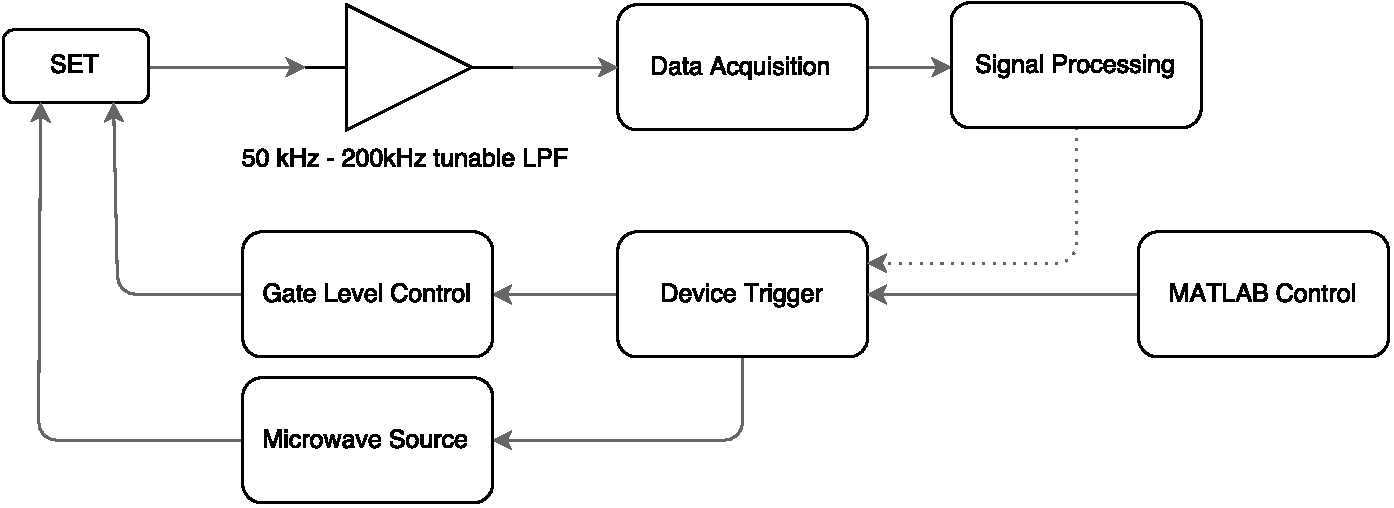
\includegraphics[width=\textwidth]{thesis_experiment.pdf}
	\caption{Block diagram of experiment}
	\label{fig::thesis_experiment}
\end{figure}


Figure \ref{fig::set_layout} shows the physical device that will be similar to one I will be testing my solution on. This devices has various voltage-controlled nodes, such as the top gate to induce a layer of electrons on the boundary, the left and right barriers to remove this layer, forming tunnel junctions to the island, and finally the plunger which can act at the gate as defined in section \ref{sec::set}.

\begin{figure}[htbp!]
	\centering
	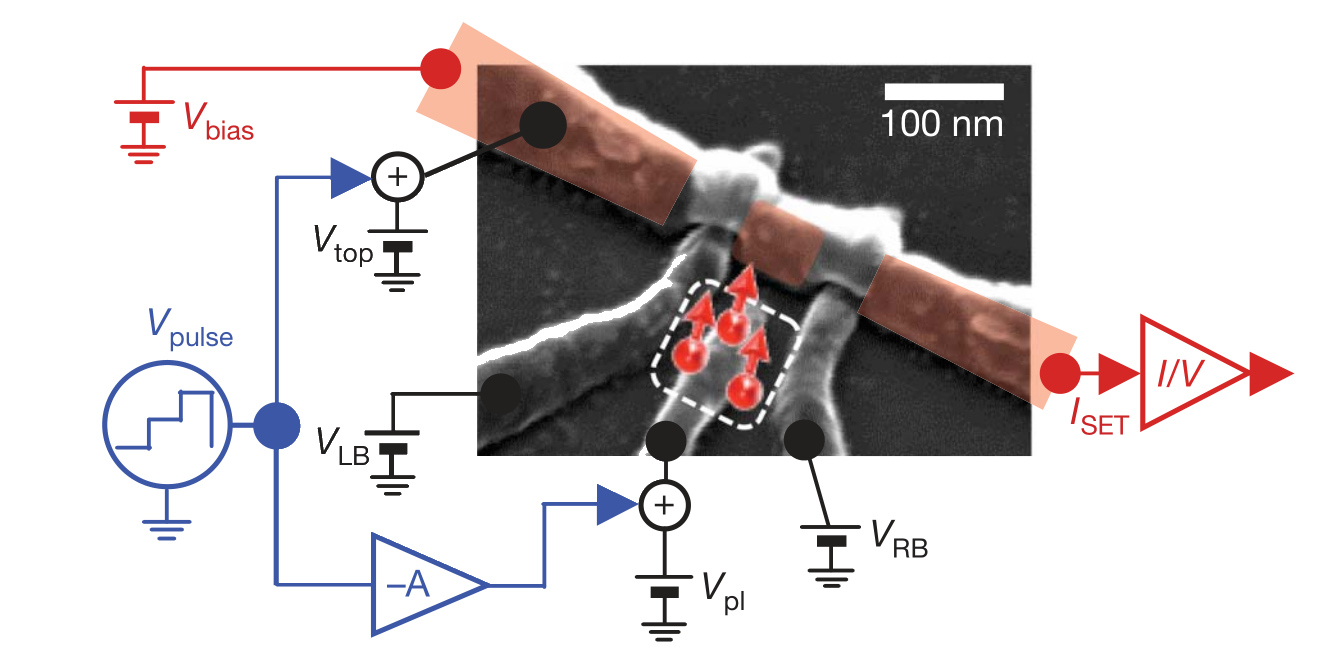
\includegraphics[width=\textwidth]{set_layout}
	\caption{The layout of an SET}
	\label{fig::set_layout}
\end{figure}

\subsection{Problem Statement}
The problem with this current approach is the cost of running these experiments if at the point of the plunge there was no electron on the donor. Any data with an incorrect initialization must be discarded, so as not to disturb the results. To take this one step further, to require 99.9\% spin-down initialization fidelity would mean ignoring over 90\% of all recorded data. This kind of waste can be circumvented by a feedback loop that can decide when the initialization has been performed correctly, and thus continue the experiment.

The problem I am to solve in this thesis is to incorporate digital feedback with current research, closing the loop in Figure \ref{fig::thesis_experiment}, which will allow for experiments to run more efficiently and lessen the burden on the researchers in selecting their data. The following section will detail some available solutions.

\subsection{Digital Devices}
\subsubsection{PCIe Digitizer Card}
%\todo[inline]{Talking points of the Digitizer solution, DMA, etc. etc.}
The ATS9440 \gls{pcie} digitizer card \cite{ATS9440} has been incorporated into the previous years' research and hence, a lot of the groundwork has been laid out for using the device, and interfacing it with experiments. It is the natural solution, to attempt to provide digital feedback in a MATLAB environment in a semi-real-time capacity. There is a clear benefit in utilizing what is already well established, conditional that it can achieve what is necessary.

The primary features of this solution are:
\begin{itemize}
	\item Range of sampling frequencies from 1 KSPS to 125 \gls{msps}
	\item 4 independent input channels
	\item Internal (from one of the 4 input channels) and external triggering
	\item 14-bit resolution, with definable input ranges of $\pm 100 \textrm{mV}$ to $\pm 4 \textrm{V}$
	\item Auto-\gls{dma} for fast storage and parallel data processing.
\end{itemize}

To verify MATLAB as a viable solution, it was first used against a full set of data that had been collected from a previous experiment. I performed a set of 3 tests, the first was to simply process the entire data in a single operation. This was the least like a real-world test, but served as a proof of concept that the peak detection, and time-out period were working. Once this was established, I moved onto performing this task on subsets, or windows, of the full data set. This is closer to a real test, and is actually extensible to the next alternative solution, as data processing on an embedded system can be limited by available memory. The test itself performed as expected, mirroring the first test. The final test was perhaps the most like a real-world solution, where I filled a circular buffer of a fixed size (512 samples) which mimics a streaming input. This allows for a near-real-time time-out detection, supposing that the time it takes to process the signal is less than the time it takes to fill a time slice of the buffer (arbitrary, 32 samples in this example). Figure \ref{fig::timeout_detection} depicts the windowed solution over a large data set.

\begin{figure}[htbp!]
	\centering
	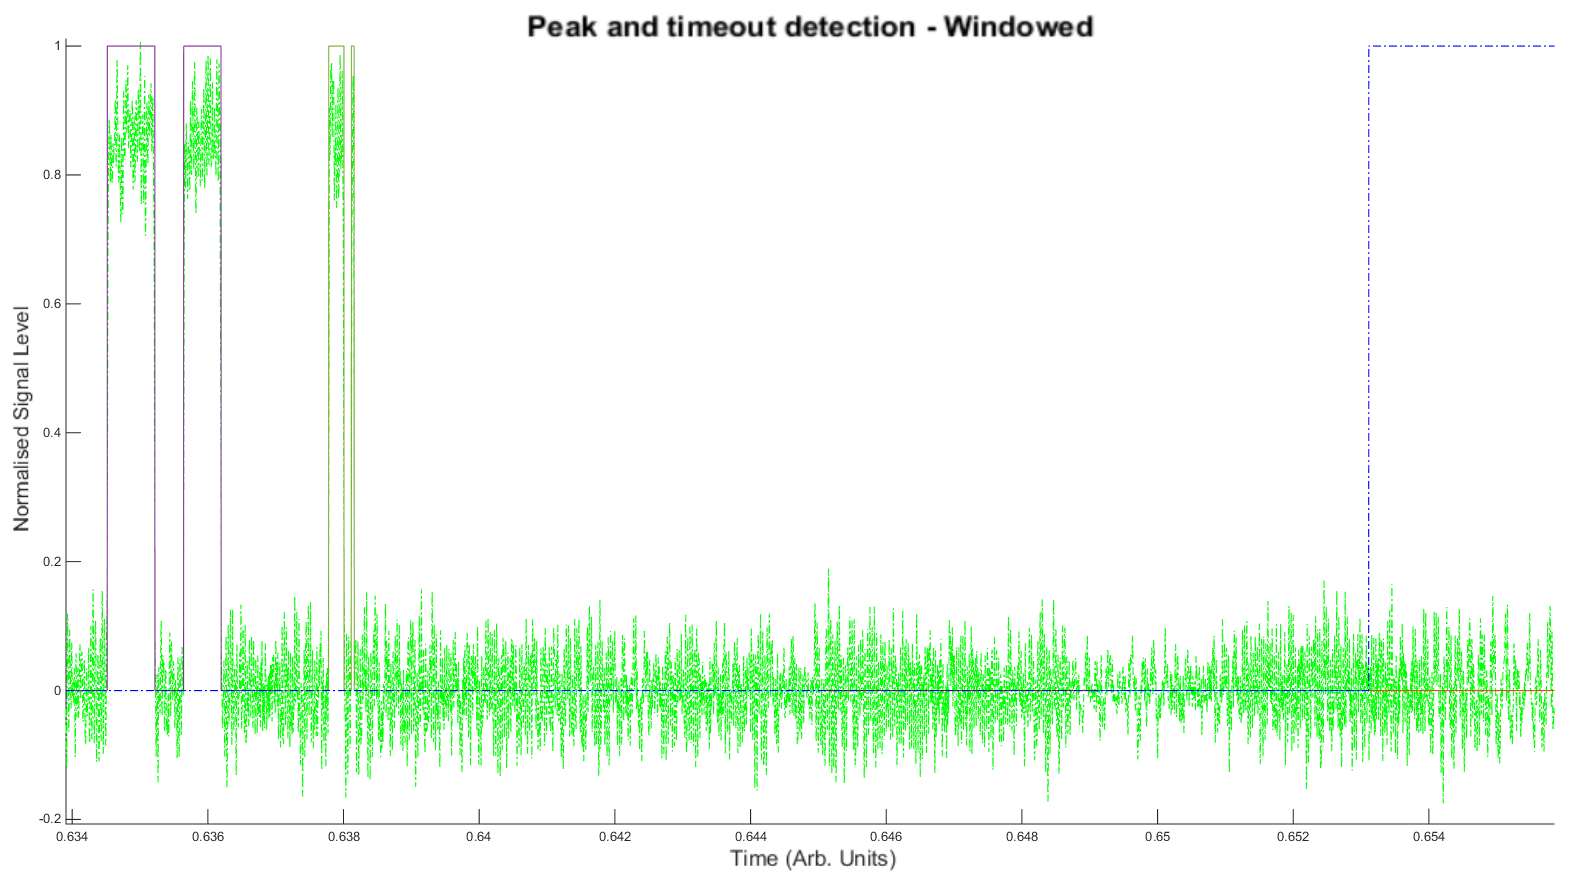
\includegraphics[width=\textwidth]{timeout_detection}
	\caption{MATLAB performing peak detection on windows of the green data set. The blue dashed line represents the output signal, once a set amount of time has passed}
	\label{fig::timeout_detection}
\end{figure}

\subsubsection{FPGA/$\mu$Controller and ADC}
%\todo[inline]{Talking points of the external FPGA and ADC solution, mention some particular examples of ADCs etc.}
An alternative solution is to have an external device which is responsible for detecting peaks in the \gls{set} current, and waiting a predetermined amount of time before setting a TTL output to high, which could then trigger the plunge, and the experiment to begin.

This approach requires the design of a high precision \gls{adc}, with a sampling rate of at least 1 MS/s. The digital data would then need to be processed by either a $\mu$Controller or a \gls{fpga}. The primary benefit of this solution is that it is versatile, and can be adapted and modified to meet different needs of the future. Furthermore, as this is completely external to the rest of the experiment, it can truly run in parallel, and accurate timing without error could prove to be more achievable.
\subsubsection{XMC}
%\todo[inline]{Talking points of the integrated XMC solution, pre-built FPGA, ADCs and possibly with Auto-DMA}
An alternative that I have recently become aware of is an integrated \gls{xmc} solution. An \gls{xmc} is another \gls{pcie} connected device, that has pluggable modules, designed for specific functions. Some are available with a high speed \gls{adc} and an on-board \gls{fpga}. This could easily circumvent the process of finding a development board for this external hardware, and could be easily re-adapted should the requirements change. These \gls{pcie} cards often come with \gls{dma} support, so this could be a good intermediate solution between the two mentioned prior.